%\documentclass[letterpaper,english,reprint,nofootinbib,aps,superscriptaddress,showpacs,showkeys]{revtex4-1}
\documentclass[prl,letterpaper,english,reprint,nofootinbib,aps,superscriptaddress,showpacs,showkeys]{revtex4-1}

\usepackage{babel,calc,amsmath,amsthm,amssymb,graphicx,subfigure,xcolor,comment}
\usepackage{mathdots}
%\usepackage[notref,notcite,color]{showkeys}
\usepackage[T1]{fontenc}
\setcounter{secnumdepth}{3}
\usepackage[unicode=true]{hyperref}
\usepackage{booktabs}
\usepackage{threeparttable}
\usepackage{braket}
\usepackage{multirow}

\usepackage[normalem]{ulem}
\hypersetup{
     colorlinks=true,       		% false: boxed links; true: colored links
     linkcolor=blue,          	% color of internal links
     citecolor=red,             % color of links to bibliography
    % filecolor=blue,      		% color of file links
     urlcolor=magenta,          % color of external links
    % runcolor=cyan
 }
%% THEOREMS -------------------------------------------------------
\newtheorem{theorem}{Theorem}
\newtheorem*{theorem*}{Theorem}
\newtheorem{corollary}{Corollary}
\newtheorem*{corollary*}{Corollary}
\newtheorem{lemma}{Lemma}
\newtheorem*{lemma*}{Lemma}
\newtheorem{proposition}{Proposition}
\newtheorem*{proposition*}{Proposition}
\theoremstyle{definition}
\newtheorem{definition}{Definition}
\newtheorem*{definition*}{Definition}
\theoremstyle{remark}
\newtheorem{remark}{Remark}
\newtheorem*{remark*}{Remark}
%% MATH -----------------------------------------------------------
\newcommand{\norm}[1]{\left\Vert#1\right\Vert}
\newcommand{\abs}[1]{\left\vert#1\right\vert}

\newcommand{\Real}{\mathbb R}
\newcommand{\eps}{\varepsilon}
\newcommand{\To}{\longrightarrow}
\newcommand{\BX}{\mathbf{B}(X)}
\newcommand{\A}{\mathcal{A}}
%% ----------------------------------------------------------------

\newcommand{\tr}{\rm tr}
\newcommand{\rom}[1]{\MakeUppercase{\romannumeral #1}}


\begin{document}
\renewcommand{\figurename}{Fig.}

\title{Experimental Demonstration of Quantum Contextuality beyond Bell Nonlocality}


\author{Zheng-Hao Liu}
\affiliation{CAS Key Laboratory of Quantum Information, University of Science and Technology of China, Hefei 230026, People's Republic of China}
\affiliation{Synergetic Innovation Center of Quantum Information and Quantum Physics, University of Science and Technology of China, Hefei 230026, People's Republic of China}

\author{Hui-Xian Meng}
\affiliation{Theoretical Physics Division, Chern Institute of Mathematics, Nankai University, Tianjin 300071, People's Republic of China}

\author{Zhen-Peng Xu}
\affiliation{Naturwissenschaftlich-Technische Fakult\"{a}t, Universit\"{a}t Siegen, Walter-Flex-Stra{\ss}e 3, 57068 Siegen, Germany}

\author{Jie Zhou}
\affiliation{Theoretical Physics Division, Chern Institute of Mathematics, Nankai University, Tianjin 300071, People's Republic of China}

\author{Sheng Ye}
\affiliation{CAS Key Laboratory of Quantum Information, University of Science and Technology of China, Hefei 230026, People's Republic of China}
\affiliation{Synergetic Innovation Center of Quantum Information and Quantum Physics, University of Science and Technology of China, Hefei 230026, People's Republic of China}

\author{Qiang Li}
\affiliation{CAS Key Laboratory of Quantum Information, University of Science and Technology of China, Hefei 230026, People's Republic of China}
\affiliation{Synergetic Innovation Center of Quantum Information and Quantum Physics, University of Science and Technology of China, Hefei 230026, People's Republic of China}

\author{Kai Sun}
\affiliation{CAS Key Laboratory of Quantum Information, University of Science and Technology of China, Hefei 230026, People's Republic of China}
\affiliation{Synergetic Innovation Center of Quantum Information and Quantum Physics, University of Science and Technology of China, Hefei 230026, People's Republic of China}

\author{Hong-Yi Su}
\affiliation{Graduate School of China Academy of Engineering Physics, Beijing 100193, People's Republic of China}

\author{Jing-Ling Chen}
\email{chenjl@nankai.edu.cn}
\affiliation{Theoretical Physics Division, Chern Institute of Mathematics, Nankai University, Tianjin 300071, People's Republic of China}

\author{Jin-Shi Xu}
\email{jsxu@ustc.edu.cn}
\affiliation{CAS Key Laboratory of Quantum Information, University of Science and Technology of China, Hefei 230026, People's Republic of China}
\affiliation{Synergetic Innovation Center of Quantum Information and Quantum Physics, University of Science and Technology of China, Hefei 230026, People's Republic of China}

\author{Chuan-Feng Li}
\email{cfli@ustc.edu.cn}
\affiliation{CAS Key Laboratory of Quantum Information, University of Science and Technology of China, Hefei 230026, People's Republic of China}
\affiliation{Synergetic Innovation Center of Quantum Information and Quantum Physics, University of Science and Technology of China, Hefei 230026, People's Republic of China}

\author{Guang-Can Guo}
\affiliation{CAS Key Laboratory of Quantum Information, University of Science and Technology of China, Hefei 230026, People's Republic of China}
\affiliation{Synergetic Innovation Center of Quantum Information and Quantum Physics, University of Science and Technology of China, Hefei 230026, People's Republic of China}

\date{\today}

\begin{abstract}
Bell nonlocality and quantum contextuality are two intrinsic properties of Nature. In this work, we compare these two fundamental concepts with the same exclusivity graph.
For Bell inequality and  the noncontextuality (NC) inequality realized in the same exclusivity graph,
 the maximum quantum violation of the NC inequality is in general larger than that of the Bell inequality. This phenomenon is called quantum contextuality beyond Bell nonlocality.
To experimentally demonstrate this phenomenon, we adopt the exclusivity graph corresponding the $I_{3322}$ inequality. Theoretically, one finds that the value of Bell nonlocality is about $6.251$, and the value of quantum contextuality is about $6.588$ for a five-dimensional system and about $6.571$ for a four-dimensional system, respectively. The gap between quantum contextuality and Bell nonlocality is about $\Delta\approx0.30$. Within the experimental errors, our experimental results coincide with the theoretical predictions.
This work would further deepen the understanding of the different kinds of quantum correlations.
\end{abstract}



\pacs{03.65.Ud, 03.67.Mn, 42.50.Xa}

	\maketitle

\emph{Introduction.}---Nonclassicality is an inherited feature that distinguishes quantum mechanics (QM) from classical theory. Among the well-known nonclassicalities, there are quantum entanglement~\cite{Horodecki}, Bell nonlocality (BN)~\cite{Bell66}, quantum contextuality (QC)~\cite{KS67} and so on. A physical theory exhibits Bell nonlocality (or lack of locality) if measurement outcomes cannot be reproduced by classical models, in which measurement outcomes are independent of the space-like separated measurements performing on some composite systems. These classical models are known as the local-hidden-variable (LHV) models. Similarly, a physical theory exhibits quantum contextuality (or lacks noncontextuality) if measurement outcomes cannot be reproduced by classical models, in which measurement outcomes are independent of the measurement context (i.e., the set of jointly measurable observables actually measured). These classical models are called  the-noncontextual-hidden variable (NCHV) models.

Bell nonlocality and quantum contextuality are two intrinsic properties of Nature. They are different concepts but closely related: (i) Both of them reflect the confliction between quantum mechanics and some types of classical models, in which measurement outcomes are determined before measurements are performed. The former refutes the LHV models, while the latter refutes the NCHV models.
%Kochen and Specker \cite{Specker60, KS67} (Bell \cite{Bell66}) already ruled out NCHV (LHV) models from quantum theory (QT).
(ii) Every Bell inequality (violation of which implies BN) becomes an NC inequality (violation of which implies QC) if the constraint of space-like separation between the compatible measurements is removed \cite{Mermin,RDLTC14}. Recently, the applications of Bell nonlocality and quantum contextuality have included speeding up quantum algorithms \cite{Howard}, fault-tolerant computation \cite{Raussendorf13}, secret key distribution \cite{Ekert91,CDNS11}, reduction of communication complexity \cite{BZPZ04,BCMW10}, and randomness certification \cite{PAMBMMOHLMM10}.

Some fundamental relations between QC and BN have been studied in the literature. For instances, the first one is the fundamental monogamy relation between contextuality and nonlocality, which was first presented in 2014~\cite{Kurzynski}, and later on was observed in the experiment~\cite{Li}. The second one refers to Bell nonlocality is tightly bounded by quantum contextuality, which can be obtained from the Cabello-Severini-Winter (CSW) graph-theoretical approach~\cite{CSW14}. The powerful CSW approach has for the first time enabled people to compare BN and QC in the same exclusivity graph: let $\Delta$ denote the gap between QC and BN, then $\Delta=0$ means Bell nonlocality saturates quantum contextuality, and $\Delta>0$ means quantum contextuality beyond Bell nonlocality. Although some theoretical examples have been provided to show that QC beyond BN~\cite{RDLTC14,SBBC13}, until now there has not been any experimental report on this subject.

The purpose of this Letter is to experimentally demonstrate quantum contextuality beyond Bell nonlocality. The crucial point is choosing an appropriate exclusivity graph, for which $\Delta$ is sufficient large such that the phenomenon of QC beyond BN can be observed in the experiment. In this work, we shall study detailedly the exclusivity graph associated to the $I_{3322}$ inequality, which gives $\Delta\approx0.3$~\cite{RDLTC14}, and then demonstrate the phenomenon of QC beyond BN by experiment. Within the experimental errors, the experimental results coincide with the theoretical predictions.

%A natural question is whether quantum contextuality may go {\em beyond} quantum nonlocality in some sense.
%One possible sense occurs within the Cabello-Severini-Winter (CSW) graph-theoretic approach to quantum contextuality \cite{CSW10,CSW14}.
%Where, corresponding to every NC or Bell inequality, there is a graph $G$ encoding the relationships of exclusivity between the events in that inequality.
%Reciprocally, given any arbitrary graph $G$, there is always a quantum system and a NC or Bell inequality with exclusivity graph $G$. The interesting thing is that the maximum NC violation is always given by a characteristic number of $G$: the Lov\'asz number of $G$. Then, does there exist a pair of NC and Bell inequalities represented by the same exclusivity graph, with the former one giving higher quantum violation?
%
%CSW already showed that the answer is positive.
%Among these cases, the $I_{3322}^{\rm CSW}\le 6$ inequality \cite{CSW10} is considered as the most interesting one. Its maximal violation is 6.58841287 for quantum contextuality, strictly higher than 6.25087538 for Bell nonlocality~\cite{Pal10}.
%The same behaviour was later observed for all bipartite Bell inequalities whose exclusivity graph is a pentagon \cite{SBBC13}. However, this case is less interesting since, unlike $I_{3322}$, these pentagonal Bell inequalities are not tight (i.e., they do not define the border that separate between local and nonlocal correlations).
%The $I_3\le 2$ inequality is another inequality exhibiting quantum contextuality beyond Bell nonlocality, and for Bell nonlocality it also defines a tight bound. However,
%the difference of maximal violation for quantum contextuality and Bell nonlocality is 0.0133, which is too small to be observed in experiment.
%
%In this Letter, we investigate the quantum contextuality and Bell nonlocality of inequality $I_{3322}^{\rm CSW}\le 6$ in four-dimensional system and two-qubits system respectively. We show that these systems are adequate for proving the phenomenon of quantum contextuality beyond Bell nonlocality, and give an experimental demonstration.
%

%Applying the (CSW) graph-theoretic approach, the $I_{3322}\le 0$ inequality proposed symmetrically in Ref.~\cite{BG08} can be rewritten as~\cite{RDLTC14}

\emph{Theory: QC beyond BN.}---To elaborate the theory clearly, let us start from the symmetric Bell inequality  $I_{3322}\le 0$~\cite{BG08}, which is a natural generalization of the well-known Clauser-Horne-Shimony-Holt inequality~\cite{CHSH} from two measurement settings to three measurement settings, and it is also tight for the two-qubit case.
The inequality can be recast to the following form~\cite{RDLTC14} (see the detail in supplementary material (SM)~\cite{SM})
 \begin{eqnarray}
 I_{3322}^{\rm CSW}
 &=&P(0,0 \vert 0,1) + P(0,0 \vert 0,2) + P(0,0 \vert 1,0) \nonumber\\
 &&+ P(0,0 \vert 1,2) + P(0,0 \vert 2,0) + P(0,0 \vert 2,1) \nonumber \\
 &&+ P(0,1 \vert 1,1) + P(1,0 \vert 1,1) + P(1,1 \vert 1,1) \nonumber\\
 &&+ P(0,1 \vert 2,2) + P(1,0 \vert 2,2) + P(1,1 \vert 2,2) \nonumber \\
 &&+ P(1,\_ \vert 0,\_) +P(1,\_ \vert 1,\_)\nonumber \\
 &&  + P(\_,1 \vert \_,0)+ P(\_,1 \vert \_,1)\stackrel{\mbox{\tiny{LHV}}}{\leq}6,
\label{I3322BL}
\end{eqnarray}
where all probabilities have positive signs, and $P(m,n|i,j)\equiv P(a_i=m, b_j=n)$ denotes the probability in which Alice's $i$-th measurement outcome is $m$ and Bob's $j$-th measurement outcome is $n$, and $P(m,\_|i,\_)\equiv P(a_i=m)$ denotes the marginal probability of Alice's $i$-th measurement result being $m$. Bell inequality (\ref{I3322BL}) is applicable for any two $d$-dimensional systems (i.e., two qudits). For two qubits, the maximal quantum violation of inequality (\ref{I3322BL}) is exactly $I_{3322}^{\rm BN}=25/4=6.25$, and the corresponding optimal observables and quantum state are given in the SM~\cite{SM} (for convenient, here we have denoted $I_{3322}^{\rm BN}$ to represent the quantum violation of Bell inequality). For two qudits, it has been shown that the maximal quantum violation $I_{3322}^{\rm BN}\approx6.25087538$ only occurs for infinite dimensional quantum systems (i.e., $d\rightarrow\infty$)~\cite{Pal10}. In other words, for the $I_{3322}$ inequality, Bell nonlocality is $I_{3322}^{\rm BN}\le 6.251$.

\begin{figure}[t]
\centering
\includegraphics[scale=0.6]{i3322.pdf}
\caption{\label{Fig7}Exclusivity graph associated with $I_{3322}^{\rm CSW}$.
The 16 vertices represent the corresponding vectors.}
\end{figure}

\begin{table}[t]
\centering
  \begin{tabular}{lccccc} \hline \hline
$|A_i\rangle$ & $i_1$ & $i_2$ & $i_3$ & $i_4$  \\
\hline
$|A_1\rangle$ & $0$ & $0$ & $1$ & $0$  \\
$|A_2\rangle$  & $0.469723$ & $0.453743$ & $0$ & $0.757283$  \\
$|A_3\rangle$ & $0.746839$ & $0.253161$ & $0$ & $0.614931$  \\
$|A_4\rangle$  & $0$ & $0.924703$ & $0$ & $-0.38069$  \\
$|A_5\rangle$ & $0.253161$ & $0.746839$ & $0$ & $-0.614931$  \\
$|A_6\rangle$ & $0.249899$ & $0.754381$ & $0$ & $0.607009$  \\
$|A_7\rangle$ & $1$ & $0$ & $0$ & $0$  \\
$|A_8\rangle$  & $0.924703$ & $0$ & $0$ & $-0.38069$  \\
$|A_9\rangle$  & $0$ & $1$ & $0$ & $0$  \\
$|A_{10}\rangle$  & $1$ & $0$ & $0$ & $0$ \\
$|A_{11}\rangle$ & $0$ & $1$ & $0$ & $0$  \\
$|A_{12}\rangle$  & $0.924703$ & $0$ & $0$ & $0.38069$  \\
$|A_{13}\rangle$  & $0$ & $0$ & $1$ & $0$  \\
$|A_{14}\rangle$  & $0$ & $0.924703$ & $0$ & $0.38069$  \\
$|A_{15}\rangle$ & $0.754381$ & $0.249899$ & $0$ & $-0.607009$  \\
$|A_{16}\rangle$  & $0.453743$ & $0.469723$ & $0$ & $0.757283$  \\
\hline
$|\psi\rangle$ & $\frac{1}{\sqrt{2}}$ & $\frac{1}{\sqrt{2}}$ & $0$ & $0$\\
  \hline \hline
   \end{tabular}
\caption{Numerically optimal measurement settings and state for $I_{3322}^{\rm QC}\approx6.57152$  in the four-dimensional system.}
\label{numerica3}
\end{table}

Then, we turn to quantum contextuality. The exclusivity graph $G$ associated with $I_{3322}^{\rm CSW}$ is shown in Fig.~\ref{Fig7}, which also appears in Ref.~\cite{RDLTC14}.
The vertices of graph $G$ represent probability events, and two connected vertices imply the two corresponding events are exclusive (or the two corresponding projectors are mutually orthogonal). Based on the exclusivity graph in Fig.~\ref{Fig7} and theorem 1 in Ref.~\cite{cabello16}, one may have the following NC inequality:
\begin{align}
I_{3322}^{\rm CSW}
&=\sum_{i\in V}P_{|\psi\rangle}(A_i=1)-\sum_{(i,j)\in E}P_{|\psi\rangle}(A_i=1,A_j=1)\nonumber\\
&\overset{{\rm{NCHV}}}\leq \beta \;\;\overset{{\rm{QM}}}\leq \vartheta(G),
\label{I3322QC}
\end{align}
where $V$ and $E$, respectively, denote the vertex and edge sets of the graph $G$,
$P_{|\psi\rangle}(A_i=1)$ denotes the probability of obtaining result 1 when the observable $|A_i\rangle\langle A_i|$ is measured on the state $|\psi\rangle $,  i.e., $P_{|\psi\rangle}(A_i=1)= |\langle \psi|A_i\rangle|^2$, $P_{|\psi\rangle}(A_i=1,A_j=1)\equiv P_{|\psi\rangle}(A_i=1)P_{|A_i\rangle}(A_j=1)$ represents experimental imprecision of $|A_i\rangle\bot |A_j\rangle$ when they are measured successively. 
The introduction of the second term into inequality (\ref{I3322QC}) is crucial and necessary: it is important to evaluate the two-point probability $P_{|\psi\rangle}(A_i=1,A_j=1)$ in order to fulfill the compatibility requirement in any contextuality test in the experiment~\cite{cabello16}. Certainly, in the ideal case the second term of probabilities becomes zero and can be neglected. In Ref.~\cite{RDLTC14}, the authors have obtained the classical bound of inequality (\ref{I3322QC}) as $\beta=6$, and also the maximal quantum violation as $I_{3322}^{\rm QC}=\vartheta(G)\approx 6.58841287$, with $\vartheta(G)$ being a characteristic number of graph $G$: the Lov\'asz number~\cite{Lovasz}. Obviously, the gap $\Delta=I_{3322}^{\rm QC}-I_{3322}^{\rm BN}\approx 0.337$ is sufficient large, therefore the $I_{3322}$
inequality is a very good candidate to experimentally demonstrate QC beyond BN.

%\emph{Remark 1}---
In SM, we show that the Lov\'asz number $\vartheta(G)\approx 6.58841287$ can be achieved in a five-dimensional system, which has not been given in~\cite{RDLTC14}, and in SM we also provide the corresponding optimal measurement settings and optimal state to detect quantum contextuality. However, to demonstrate the phenomenon of QC beyond BN in experiment, it is sufficient to consider the four-dimensional quantum system (instead of a five-dimensional system), for which the maximal quantum contextuality is only slightly smaller than the Lov\'asz number, i.e., $I_{3322}^{\rm QC}\approx6.57152$. The optimal settings and the state are listed in Table~\ref{numerica3}, and the orthogonal relationship can be satisfied with errors of $10^{-32}$ magnitude, i.e., $\sum_{(i,j)\in E}P_{|\psi\rangle}(A_i=1,A_j=1)\approx 9.62965\times 10^{-33}<10^{-32}$. In this case, the gap $\Delta=I_{3322}^{\rm QC}-I_{3322}^{\rm BN}\approx 0.320$, which is enough to indicate QC beyond BN.



\begin{figure*}[t]
    \centering
    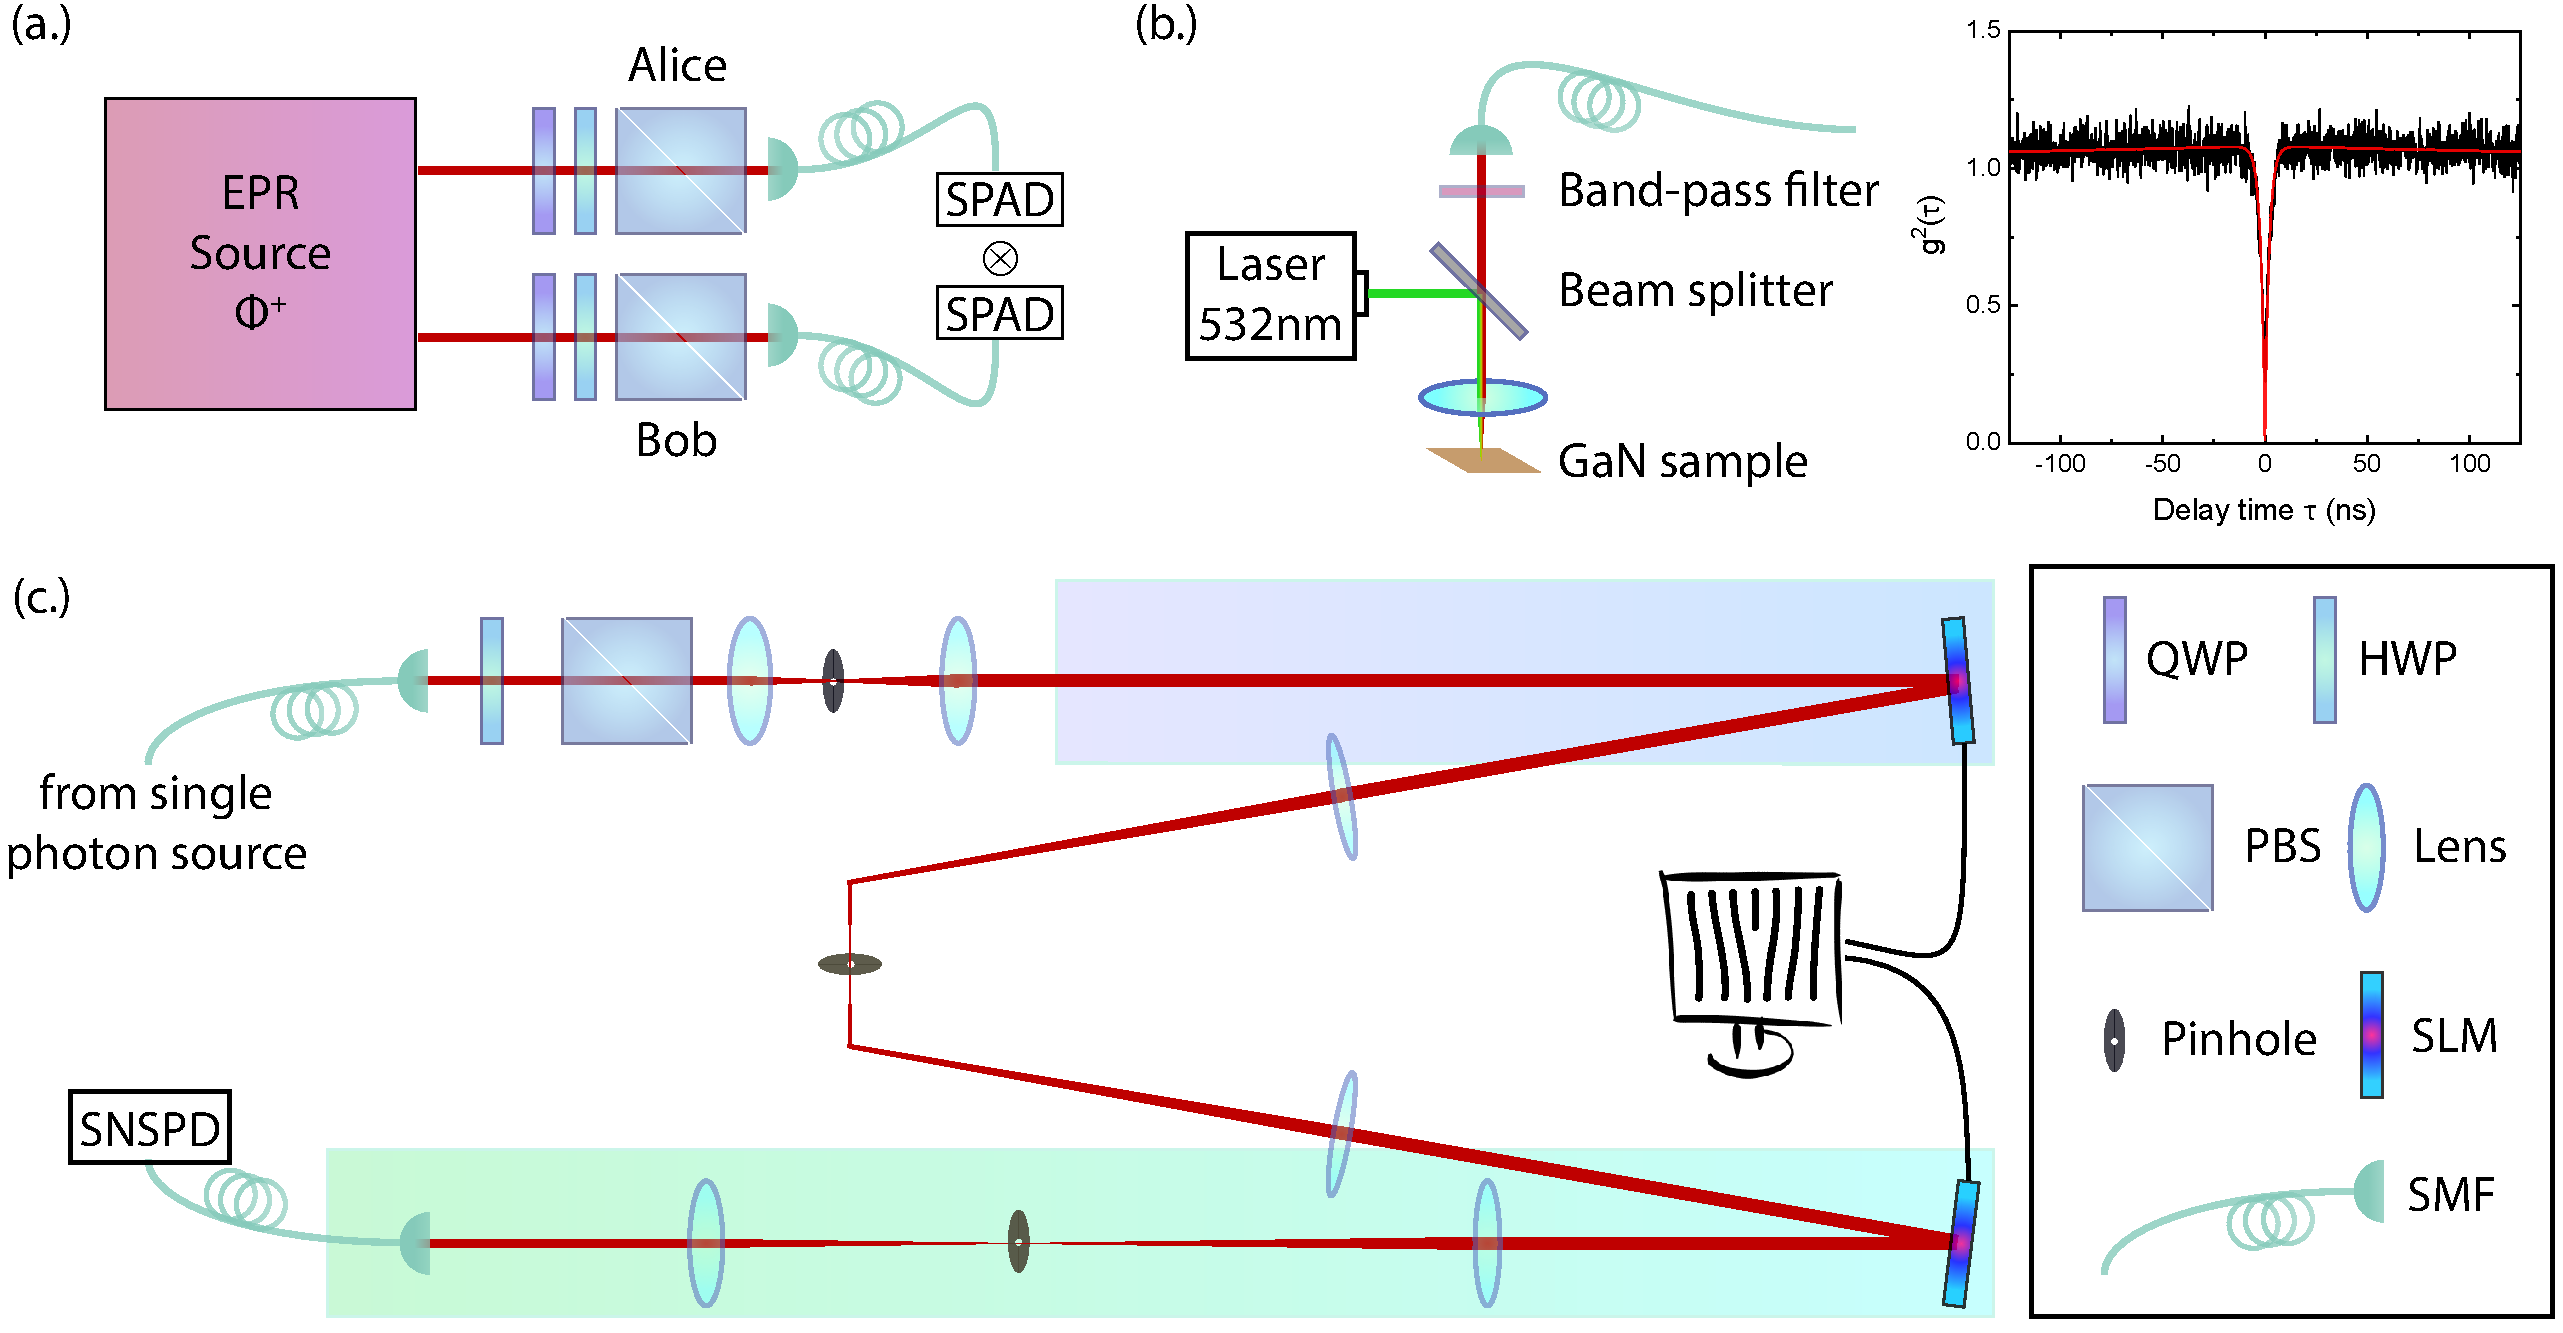
\includegraphics[width=160mm]{fig/exp-sch-draft-v2.pdf}
    \caption{(color online). Experimental setup.
    (a.) The two-particle setup to check Bell nonlocality. Two maximally polarization-entangled photons were separately sent to Alice and Bob, going through their polarization discrimination system and recorded by single-photon avalanche detectors (SPAD).
    (b.) The single photon source, prepared by exciting an intrinsic defect in a bulk GaN sample. The second-order photon correlation function at zero delay without background correction was 0.225, clearly exhibiting the signature of photon antibunching and confirmed the character of single-photon emission. Single photons were further filtered by a band-pass filter with a central wavelength of 780 nm and a bandwidth of 25 nm, and sent to the contextuality test setup.
    (c.) The single-body contextuality test setup.
    %Single photons filtered by a single mode optical fiber (SMF) were sent to the setup.     The polarization of single photon was prepared by a half-wave plate (HWP) and a polarization beam splitter (PBS).
    The single photons from (b), after passing through the beam expanding system with two lenses and a pinhole between them, were sent to a spatial light modulator (SLM) controlled by a computer to prepared the high-dimensional states, which is denoted by an violet box. The measurement setup consists of another SLM and single mode fiber (SMF), and the counting apparatus here was a superconducting nanowire single-photon detector (SNSPD).}
    \label{fig:exp-sch}
 \end{figure*}

%\emph{Remark 2}---For the optimal settings and state, the orthogonal relationship can be satisfied with errors of $10^{-32}$ magnitude, i.e.,
%$\sum_{(i,j)\in E}P_{|\psi\rangle}(A_i=1,A_j=1)\approx 9.62965\times 10^{-33}<10^{-32}.$
%In fact, there exist settings and state such that the orthogonal relationship is strictly satisfied  (i.e., $\sum_{(i,j)\in E}P_{|\psi\rangle}(A_i=1,A_j=1)=0$) and $\max I_{3322}^{\rm QC}\approx 6.56233.$ For the detail, see Ref.~\cite{SM}.

Since the quantum system we utilize in experiment is four-dimensional, we need to extend the graph with extra projectors to construct full sets of compatible observables, such that every projector is measured as part of a complete basis \cite{yxiao17}. By Table~\ref{numerica3}, we only need to measure with the following six complete bases:
\begin{eqnarray}
\left\{
  \begin{array}{ll}
    \{|A_1\rangle,|A_2\rangle,|A_3\rangle,|A_{17}\rangle\},  \{|A_1\rangle,|A_4\rangle,|A_7\rangle,|A_{18}\rangle\},\\
\{|A_1\rangle,|A_{5}\rangle,|A_{16}\rangle,|A_{19}\rangle\},
\{|A_1\rangle,|A_{9}\rangle,|A_{12}\rangle,|A_{20}\rangle\},\ \ \ \\
\{|A_{6}\rangle,|A_{8}\rangle,|A_{21}\rangle,|A_{22}\rangle\},
\{|A_{14}\rangle,|A_{15}\rangle,|A_{23}\rangle,|A_{24}\rangle\},
\end{array}
\right.
\end{eqnarray}
where $|A_{21}\rangle$ and $|A_{23}\rangle$ can be taken as $|A_{1}\rangle$, and $|A_{17}\rangle,|A_{18}\rangle,|A_{19}\rangle,|A_{20}\rangle,|A_{22}\rangle,|A_{24}\rangle$ are uniquely determined by their corresponding incomplete basis since the system we focus on is four-dimensional and the all incomplete bases have three pairwise orthogonal vectors.
 Thus, the detection probability of each observable, such as $|A_{2}\rangle\langle A_{2}|$, can be obtained as $P_{|\psi\rangle}(A_2=1)=
{N_{|\psi\rangle}(A_2)}/[N_{|\psi\rangle}(A_1)+N_{|\psi\rangle}(A_2)+N_{|\psi\rangle}(A_3)+N_{|\psi\rangle}(A_{17})]$,
%\begin{eqnarray}
%\begin{split}
%&P_{|\psi\rangle}(A_2=1)=\\
%&\frac{N_{|\psi\rangle}(A_2)}
%{N_{|\psi\rangle}(A_1)+N_{|\psi\rangle}(A_2)+N_{|\psi\rangle}(A_3)+N_{|\psi\rangle}(A_{17})},
%\end{split}
%\end{eqnarray}
where $N_{|\psi\rangle}(A_i)$ is the number of counts of obtaining result 1 when the observable $|A_{i}\rangle\langle A_{i}|$ is measured on the state $|\psi\rangle.$


  \begin{figure*}[htbp]
     \centering
     \includegraphics[width =160mm]{fig/exp-res-all.pdf}
     \caption{(color online).Experimental results of detection probabilities for computing $I_{3322}^{BN}$ (a) and $I_{3322}^{QC}$ (b and c).
     \label{fig:exp-res-all}
     (a) Coincidence counting probabilities of Alice and Bob when they choose their optimal settings.
     \label{fig:exp-res-all}
     (b) Detection probabilities of the 16 optimal projectors, representing the 16 vertices of corresponding exclusivity graph, with the input state $|\psi\rangle$.
     The dots are arranged in $(xyz)\to(|\braket{i_1|\psi}|^2, |\braket{i_2|\psi}|^2, \braket{i_4|\psi}|\braket{i_4|\psi}|)$ direction and the third dimension of $\braket{i_3|\psi}$ is omitted, so that $\braket{1|\psi}$ and $\braket{13|\psi}$ fall at the origin of Cartesian coordinate and are hidden, in which the experimental results also agree well with the theoretical prediction.
     \label{fig:exp-res-all}
     (c) Detection probabilities of nonzero $P_{\ket{\alpha_i}}(\alpha_j=1)$, where eigenstates $\ket{\alpha_i}$ and projectors $\ket{\alpha_j}\bra{\alpha_j}$ are denoted by vertices, connected by 32 edges in the exclusivity graph.
     }
 \end{figure*}




 \emph{Experimental Setup and Result.---}We are now ready to experimentally test the two distinct quantum values of $I^{\rm CSW}_{3322}$, namely, $I_{3322}^{\rm BN}\leq6.251$ and $I_{3322}^{\rm QC}\leq6.571$ separately, to explicitly demonstrate quantum contextuality beyond Bell nonlocality. The experimental setup is illustrated in Fig.~\ref{fig:exp-sch}. We start from $I_{3322}^{\rm BN}$. Based on the maximally entangled state $\ket{\Phi^+}=(|00\rangle+|11\rangle)/\sqrt{2}$ of two photonic polarization qubits, we checked the maximal violation of inequality (\ref{I3322BL}).
 A type-\rom{2} $\beta$-Barium borate ($\beta$-BBO) crystal was pumped by a frequency-doubled femtosecond laser to generate  polarization-entangled biphoton, which were further sent to Alice and Bob, where a polarization beam splitter (PBS), proceeded by a quarter waveplate (QWP) and a half waveplate (HWP), was utilized to construct a polarization discrimination system.
 Two single-photon avalanche detectors (SPAD) recorded photon counting rate after the polarization discrimination system, and their coincidence counts was proportional to the probability of detecting two photons with a certain setting.

 %In the two-dimensional case, the setting to acquire maximal possible violation with two maximally entangled qubits $\ket{\Phi^+}$ have been worked out. More precisely, these settings are listed in table~\ref{tab:set3}.
For each set of measurement, the total photon count was about $8000$, and result was shown in Fig.~\ref{fig:exp-res-all}a. Substituting the measurement result into (\ref{I3322BL}) gives a result of $I_{3322}^{BN}=6.165 \pm 0.012$. Here, the errors were calculated according to the Poisson distribution, more precisely, by simulating the values of each measurement quantity from Poisson distribution for 100 randomly groups of counting sets, and taking the standard deviation of the simulated results as error. The result surpasses prediction of any possible LHV model but, due to imperfections in experiment, falls sightly below two qubit's Tsirelson bound $6.25$.

 We now turn to inspection of $I_{3322}^{\rm QC}$. In a four-dimensional space, the single-body quantum contextual violation of the inequality (\ref{I3322QC}) was checked.
 To construct this synthetic space, we exploit the capability of the orbital angular momentum (OAM) of light. Unlike photon's polarazation which is a homomorphic of a two-state system, OAM ideally spans an infinite dimension space, and the eigenstates with lower winding numbers allow precise manipulation.
 The manipulation of states was accomplished by modulating the phase of the photon's wavefunction.

 By exciting an intrinsic defect in a bulk GaN sample, we obtained an ultrabright, photostable single-photon sources at room temperature~\cite{qli18}.
 A band-pass filter with a central wavelength of 780 nm and a width of 25 nm was inserted to filter the fluorescence of the defects and match the operation wavelength of the contextuality test setup. The total photon counting rate post the filter was about $0.94M$cps.

 The single photon was directed to the setup by a single-mode fiber (SMF), and spatial-filtered into fundamental Gaussian mode.
 Using a spatial light modulator (SLM), a coordinate-related wavefunction, determined by holograms displayed on the SLM, was bestowed to photons.
 The photons would then carry a wavefunction resembling superpositions of Laguerre-Gaussian modes $LG_p^l$ with OAM number of $l$~\cite{allen92} and be prepared to desired initial four-dimensional states $\ket{\psi}$, after being diffracted by the first SLM. The four eigenvectors are set to be $\ket{i_1} = \ket{1}, \ket{i_2} = \ket{3}, \ket{i_3} = \ket{-1}$
 A $4f$ system mapped the first and the second SLM at its input and output plane, with an aperture inserted at the focal plane to filter off the unwanted zero- and higher-order diffraction terms.
 The second SLM converted specific basis $\ket{\alpha}$ back to $\ket{0}$, which was post-selected by a SMF, as photons carrying nonzero OAM cannot be focused to a spot and collected by a SMF.
 In addition, a telescope lens was inserted between the second SLM and SMF to adjust beam size and optimize fiber coupling efficiency.
 Photons were then sent to a superconducting nanowire single-photon detector (SNSPD), where the counting rate would be proportional to the probability of projection measurements, i.e., $\left|\braket{\alpha|\psi}\right|^2$.

 The input state was prepared to be $\ket{\psi} = (\ket{i_1}+\ket{i_2})/\sqrt{2}$, and the 16 corresponding projectors $\bra{A_j}(j=1,2,\cdots,16)$ were then measured on 6 sets of complete bases.
 We further considered the experimental imperfections. Orthogonality of states represented by connected vertices in the exclusivity graph was tested, and their effects were subtracted, yielding the second term of $I_{3322}^{\rm QC}$.
 To test the inequality~(\ref{I3322QC}), we also need to check the no-signaling condition, which requires the local marginal probabilities of successive measurements to be irrelevant to the other settings, forward or backward in time, being chosen, as suggested in~\cite{cabello16}. See~\cite{SM} for detailed information of this test.

 The first term of $I_{3322}^{QC}$ inequality was evaluated by directly referring to detect probabilities of the 16 corresponding projectors on $6$ full sets of compatible observables. In order to obtain all probabilities needed for the exclusivity graph, there were 19 independent projectors in total.
 Measurement settings of these projectors were shown in~\cite{SM}.
 The counting rate of each projector was then recorded and the detection probability was calculated. The integration time for each projection measurement was 10 seconds. Shown in Fig.~\ref{fig:exp-res-all}b, the results were fairly close to prediction.
 The experimental result of the first term of $I_{3322}^{QC}$ was $6.548 \pm 0.020$, error estimated by assuming Poisson distribution.

\iffalse

\begin{table}[htbp]
    \centering
    \begin{tabular}{|c|cccc|} \hline \hline
$\ket{i}$ & $i_1$ & $i_2$ & $i_3$ & $i_4$  \\
\hline
$\ket{1}, \ket{13}, \ket{21}, \ket{23}$ & $0$ & $0$ & $1$ & $0$  \\
$|2\rangle$  & $0.469723$ & $0.453743$ & $0$ & $0.757283$  \\
$|3\rangle$ & $0.746839$ & $0.253161$ & $0$ & $0.614931$  \\
$|4\rangle$  & $0$ & $0.924703$ & $0$ & $-0.38069$  \\
$|5\rangle$ & $0.253161$ & $0.746839$ & $0$ & $-0.614931$  \\
$|6\rangle$ & $0.249899$ & $0.754381$ & $0$ & $0.607009$  \\
$\ket{7}, \ket{10}$ & $1$ & $0$ & $0$ & $0$  \\
$|8\rangle$  & $0.924703$ & $0$ & $0$ & $-0.38069$  \\
$\ket{9}, \ket{11}$  & $0$ & $1$ & $0$ & $0$  \\
$|12\rangle$  & $0.924703$ & $0$ & $0$ & $0.38069$  \\
$|14\rangle$  & $0$ & $0.924703$ & $0$ & $0.38069$  \\
$|15\rangle$ & $0.754381$ & $0.249899$ & $0$ & $-0.607009$  \\
$|16\rangle$  & $0.453743$ & $0.469723$ & $0$ & $0.757283$  \\
$\ket{17}$ & $0.470735$ & $-0.854416$ & $0$ & $-0.219958$ \\
$\ket{18}$ & $0$ & $0.38069$ & $0$ & $0.924703$ \\
$\ket{19}$ & $0.854416$ & $-0.470735$ & $0$ & $-0.219958$ \\
$\ket{20}$ & $0.38069$ & $0$ & $0$ & $-0.924703$ \\
$\ket{22}$ & $0.287185$ & $-0.656437$ & $0$ & $0.697578$ \\
$\ket{24}$ & $0.656437$ & $-0.287185$ & $0$ & $0.697578$ \\
\hline
$|\psi\rangle$ & $1/\sqrt{2}$ & $1/\sqrt{2}$ & $0$ & $0$ \\
  \hline \hline
   \end{tabular}
    \caption{Measurement settings for $I_{3322}^{QC}$ in four-dimensional systems to acquire maximal violation against NCHV models.}
    \label{tab:set19}
 \end{table}

\fi

 The second term of $I_{3322}^{\rm QC}$ inequality which represents experimental imperfections of orthogonality between states denoted by connected vertices in the exclusivity graph.
 Similar as the way the first term was calculated, the second term was also evaluated by adding up mutual projection probabilities of the states mentioned above, and their fluctuation also estimated by Poisson distribution. The measurement result is shown in Fig.~\ref{fig:exp-res-all}c, yielding a value of $-0.060 \pm 0.005$ without correcting background noise from SNSPD and stray light.

 By adding the two terms together, the final result of quantum contextuality is $I_{3322}^{\rm QC}=6.488 \pm 0.025$, exceeding the classical bound by about 19 standard deviations and the Tsirelson bound derived from Bell nonlocality by over 9 standard deviations. We thus successfully observed the quantum contextuality beyond Bell nonlocality.

 \emph{Conclusion.}---In conclusion, we have compared Bell nonlocality and quantum contextuality in the same exlusivity graph associated to the $I_{3322}$ inequality. Quantum contextuality has been investigated in both five- and four-dimensional systems, and we find that the gap between contextuality and nonlocality is about $0.3$. We also perform experiment to demonstrate the phenomenon of QC beyond BN. Within the experimental errors, our results coincide with the theoretical predictions.
  %The inequality approach is a lucid method to describe the degree how contextual and nonlocal QT is. By virtue of graph theory, connections between quantum contextuality and graph's characteristic Lov\'asz number is established.
% Following the CSW approach, we have investigated the exclusivity graph which gives $I_{3322}$ inequality.
% By removing the constraints of Bell-type experiment, for the $I_{3322}$ case a remarkably high violation from any non-contextual hidden variable model exists, which cannot be explained by nonlocality per se, and has to be accounted for by quantum contextuality.
% The key point lays under this result is that, although quantum contextuality is stated without spacelike restriction, and may be considered a more weakened property than Bell nonlocality, it actually gives stronger prediction in some sense.
 Our work indicate the deep-rooted connection between graph theory and nonclassicality, and is in turn beneficial for profound comprehension of quantum mechanics.


%\begin{acknowledgments}
 \textit{Acknowledgement}.---This work was supported by the National Key Research and Development Program of China (Grant No. 2016YFA0302700), the National Natural Science Foundation of China (Grants No. 61725504, 61327901, 61490711 and 11774335), the Key Research Program of Frontier Sciences, Chinese Academy of Sciences (CAS) (Grant No. QYZDY-SSW-SLH003), Anhui Initiative in Quantum Information Technologies (AHY060300 and AHY020100), the Fundamental Research Funds for the Central Universities (Grant No. WK2470000020 and WK2470000026). H.X.M. was supported by the Project funded by China Post-doctoral Science Foundation (No. 2018M631726). J.L.C. is supported by National Natural Science Foundations of China (Grant No.\ 11475089) and the Fundamental Research Funds for the Central Universities, Nankai University(Grant No.\ 63191507). The processing of GaN sample was partially carried out at the USTC Center for Micro and Nanoscale Research and Fabrication.

 Z.H.L., H.X.M. and Z.P.X. contributed equally to this work.
%\end{acknowledgments}



\begin{thebibliography}{10}
%	\providecommand{\url}[1]{\texttt{#1}}
%	\providecommand{\urlprefix}{URL }
%	\providecommand{\eprint}[2][]{\url{#2}}
%\bibitem{Specker60}
% E. P. Specker,
% %Die Logik nicht gleichzeitig entscheidbarer Aussagen.
% \href{http://onlinelibrary.wiley.com/doi/10.1111/j.1746-8361.1960.tb00422.x/abstract}{Dialectica \textbf{14}, 239 (1960).}

 \bibitem{Horodecki}
R.~Horodecki, P.~Horodecki, M.~Horodecki, and K.~Horodecki,
 \href{https://journals.aps.org/rmp/pdf/10.1103/RevModPhys.81.865}
%Quantum entanglement,
 {Rev.~Mod.~Phys. \textbf{81}, 865 (2009).}


\bibitem{Bell66}
 J. S. Bell,
 %On the problem of hidden variables in quantum mechanics.
 \href{http://rmp.aps.org/abstract/RMP/v38/i3/p447_1}{Rev. Mod. Phys. \textbf{38}, 447 (1966).}


\bibitem{KS67}
 S. Kochen and E. P. Specker,
 %The problem of hidden variables in quantum mechanics.
 \href{http://www.iumj.indiana.edu/IUMJ/fulltext.php?year=1968&volume=17&artid=17004}{J. Math. Mech. \textbf{17}, 59 (1967).}


\bibitem{Mermin}
N. D. Mermin,
%Simple Unified Form for the Major No-Hidden-Variables Theorems,
\href{https://journals.aps.org/prl/pdf/10.1103/PhysRevLett.65.3373}
{Phys. Rev. Lett. \textbf{65}, 3373 (1990).}

\bibitem{RDLTC14}
 R. Rabelo, C. Duarte, A. J. L\'opez-Tarrida, M. Terra Cunha, and A. Cabello,
 %Multigraph approach to quantum nonlocality.
 \href{https://iopscience.iop.org/article/10.1088/1751-8113/47/42/424021/meta}
 {J. Phys. A: Math. Theor. \textbf{47}, 424021 (2014).}






%\bibitem{Bell64}
% J. S. Bell,
% Physics \textbf{1}, 195 (1964).
%
%%%%%%%%%%%%%%%%%%%%%%%%%%%%%%%%%%%%%%%%%%%%%%%%%%%%%%%%%%%%%%%%%%%%
%
%\bibitem{KCBS08}
% A. A. Klyachko, M. A. Can, S. Binicio\u{g}lu, and A. S. Shumovsky,
% %Simple Test for Hidden Variables in Spin-1 Systems
% \href{http://dx.doi.org/10.1103/PhysRevLett.101.020403}{Phys. Rev. Lett. \textbf{101}, 020403 (2008).}
%
%\bibitem{Cabello08}
% A. Cabello,
% %Experimentally Testable State-Independent Quantum Contextuality.
% \href{http://dx.doi.org/10.1103/PhysRevLett.101.210401 }{Phys. Rev. Lett. \textbf{101}, 210401 (2008).}

%%%%%%%%%%%%%%%%%%%%%%%%%%%%%%%%%%%%%%%%%%%%%%%%%%%%%%%%%%%%%%%%%%%


%%%%%%%%%%%%%%%%%%%%%%%%%%%%%%%%%%%%%%%%%%%%%%%%%%%%%%%%%%%%%%%%%%%

\bibitem{Howard} M. Howard, J. Wallman, V. Veitch, and J. Emerson,
\href{https://www.nature.com/articles/nature13460}
{Nature (London) \textbf{510}, 351 (2014).}




\bibitem{Raussendorf13}
 R. Raussendorf,
 %Contextuality in measurement-based quantum computation.
 \href{http://link.aps.org/doi/10.1103/PhysRevA.88.022322}{Phys. Rev. A \textbf{88}, 022322 (2013).}



%%%%%%%%%%%%%%%%%%%%%%%%%%%%%%%%%%%%%%%%%%%%%%%%%%%%%%%%%%%%%%%%%%%

\bibitem{Ekert91}
 A. K. Ekert,
 %Quantum cryptography based on Bell's theorem.
 \href{http://journals.aps.org/prl/abstract/10.1103/PhysRevLett.67.661}{Phys. Rev. Lett. \textbf{67}, 661 (1991).}

\bibitem{CDNS11}
 A. Cabello, V. D'Ambrosio, E. Nagali, and F. Sciarrino,
 %Hybrid ququart-encoded quantum cryptography protected by Kochen-Specker contextuality.
 \href{http://journals.aps.org/pra/abstract/10.1103/PhysRevA.84.030302}{Phys. Rev. A \textbf{84}, 030302(R) (2011).}

%%%%%%%%%%%%%%%%%%%%%%%%%%%%%%%%%%%%%%%%%%%%%%%%%%%%%%%%%%%%%%%%%%%

\bibitem{BZPZ04}
 \v{C}. Brukner, M. \.{Z}ukowski, J.-W. Pan, and A. Zeilinger,
 %Bell's inequalities and quantum communication complexity.
 \href{http://journals.aps.org/prl/abstract/10.1103/PhysRevLett.92.127901}{Phys. Rev. Lett. \textbf{92}, 127901 (2004).}

\bibitem{BCMW10}
 H. Buhrman, R. Cleve, S. Massar, and R. de Wolf,
 %Nonlocality and communication complexity.
 \href{http://journals.aps.org/rmp/abstract/10.1103/RevModPhys.82.665}{Rev. Mod. Phys. \textbf{82}, 665 (2010).}

%%%%%%%%%%%%%%%%%%%%%%%%%%%%%%%%%%%%%%%%%%%%%%%%%%%%%%%%%%%%%%%%%%%

\bibitem{PAMBMMOHLMM10}
 S. Pironio, \emph{et al.},
 %A. Ac\'{\i}n, S. Massar, A. Boyer de la Giroday,  D. N. Matsukevich, P. Maunz, S. Olmschenk, D. Hayes, L. Luo, T. A. Manning, and C. Monroe,
 %Random numbers certified by Bell's theorem.
 \href{http://www.nature.com/nature/journal/v464/n7291/full/nature09008.html}{Nature (London) \textbf{464}, 1021 (2010).}

%\bibitem{UZZWYDDK13}
% M. Um, X. Zhang, J. Zhang, Y. Wang, S. Yangchao, D.-L. Deng, L.-M. Duan, and K. Kim,
% %Experimental certification of random numbers via quantum contextuality.
% \href{http://www.nature.com/srep/2013/130409/srep01627/full/srep01627.html}{Sci. Rep. \textbf{3}, 1627 (2013).}

 \bibitem{Kurzynski}
P.~Kurzy${\rm \acute{n}}$ski, A.~Cabello, and D.~Kaszlikowski,
 \href{https://journals.aps.org/prl/pdf/10.1103/PhysRevLett.112.100401}
%Fundamental Monogamy Relation between Contextuality and Nonlocality,
{Phys. Rev. Lett. \textbf{112}, 100401 (2014).}


\bibitem{Li}
T.~Li, X.~Zhang, Q.~Zeng, B.~Wang, and X.~D.~Zhang,
%Experimental simulation of monogamy relation between contextuality and nonlocality in classical light,
\href{https://www.osapublishing.org/DirectPDFAccess/75609127-9CAD-CE26-93F0FBF2C26787E3_385890/oe-26-9-11959.pdf?da=1&id=385890&seq=0&mobile=no}
{Opt.~Express \textbf{26}, 9 (2018).}


%%%%%%%%%%%%%%%%%%%%%%%%%%%%%%%%%%%%%%%%%%%%%%%%%%%%%%%%%%%%%%%%%%%


%\bibitem{CSW10}
% A. Cabello, S. Severini, and A. Winter,
% %(Non-)Contextuality of physical theories as an axiom.
% \href{http://arxiv.org/abs/1010.2163}{\eprint{arXiv:1010.2163}.}

\bibitem{CSW14}
 A. Cabello, S. Severini, and A. Winter,
 %Graph-theoretic approach to quantum correlations
 \href{http://journals.aps.org/prl/abstract/10.1103/PhysRevLett.112.040401}{Phys. Rev. Lett. \textbf{112}, 040401 (2014).}


 \bibitem{SBBC13}
 M. Sadiq, P. Badzi{\c a}g, M. Bourennane, and A. Cabello,
 %Bell inequalities for the simplest exclusivity graph.
 \href{http://pra.aps.org/abstract/PRA/v87/i1/e012128}{Phys. Rev. A \textbf{87}, 012128 (2013).}

 \bibitem{BG08}
 N. Brunner and N. Gisin,
 %Partial list of bipartite Bell inequalities with four binary settings.
 \href{http://dx.doi.org/10.1016/j.physleta.2008.01.052}{Phys. Lett. A \textbf{372}, 3162 (2008).}


 \bibitem{CHSH}
J. F. Clauser, M. A. Horne, A. Shimony, and R. A. Holt,
%Proposed Experiment to Test Local Hidden-Variable Theories,
\href{https://journals.aps.org/prl/abstract/10.1103/PhysRevLett.23.880}{Phys. Rev. Lett. \textbf{23}, 880 (1969)}.


\bibitem{SM}
See \href{https://journals.aps.org/} {Supplementary Material} for detailed proofs.


\bibitem{Pal10}
 K. F. P\'al and T. V\'ertesi,
 %Maximal violation of the I3322 inequality using infinite dimensional quantum systems.
 \href{https://dx.doi.org/10.1103/PhysRevA.82.022116}{\eprint{Phys. Rev. A 82, 022116 (2010)}.}


%%%%%%%%%%%%%%%%%%%%%%%%%%%%%%%%%%%%%%%%%%%%%%%%%%%%%%%%%%%%%%%%%%%








\bibitem{cabello16}
 A.~Cabello,
 %Simple method for experimentally testing any form of quantum contextuality,
 \href{https://journals.aps.org/pra/pdf/10.1103/PhysRevA.93.032102}
 {Phys.~Rev.~A, \textbf{93}, 032102 (2016).}

\bibitem{Lovasz}
L. Lov\'asz,
%¡°On the Shannon capacity of a graph,¡±
IEEE Trans. Inf. Theory \textbf{25}, 1¨C7 (1979).

\bibitem{yxiao17}
 Y.~Xiao, \emph{et al.},
 %Z.-P.~Xu, Q.~Li, J.-S.~Xu, K.~Sun, J.-M.~Cui, Z.-Q.~Zhou, H.-Y.~Su, A.~Cabello, J.-L.~Chen, C.-F.~Li, and G.-C.~Guo,
 %Experimental observation of quantum state-independent contextuality under no-signaling conditions,
 \href{https://www.osapublishing.org/oe/abstract.cfm?uri=oe-26-1-32}
 {Opt.~Express \textbf{26} 38 (2018).}

 \bibitem{qli18}
 Q.~Li, et al.,
 \href{https://www.osapublishing.org/optica/abstract.cfm?uri=optica-6-1-67&origin=search}
 %Experimental simulation of anti-parity-time symmetric Lorentz dynamics,
 {Optica \textbf{6}, 67 (2019).}

% \bibitem{bolduc13}
% E.~Bolduc, N.~Bent, E.~Santamato, E.~Karimi, and R.~W.~Boyd,
% Exact solution to simultaneous intensity and phase encryption with a single phase-only hologram,
% Opt.~Lett. \textbf{38}, 3546 (2013).

 \bibitem{allen92}
 L.~Allen, M.~W.~Beijersbergen, R.~J.~C.~Spreeuw, and J.~P.~Woerdman,
 \href{https://journals.aps.org/pra/pdf/10.1103/PhysRevA.45.8185}
 %Orbital angular momentum of light and the transformation of Laguerre-Gaussian laser modes,
 {Phys.~Rev.~A \textbf{45}, 8185 (1992).}

 %\bibitem{mair01}
 %A.~Mair, A.~Vaziri, G.~Weihs, and A.~Zeilinger,
 %Entanglement of the orbital angular momentum states of photons,
 %Nature \textbf{412} 313 (2001).







\end{thebibliography}


\end{document}



